\documentclass[conference]{IEEEtran}
\IEEEoverridecommandlockouts
% The preceding line is only needed to identify funding in the first footnote. If that is unneeded, please comment it out.
\usepackage{cite}
\usepackage{amsmath,amssymb,amsfonts}
\usepackage{algorithmic}
\usepackage{graphicx}
\usepackage{textcomp}
\usepackage{xcolor}
\def\BibTeX{{\rm B\kern-.05em{\sc i\kern-.025em b}\kern-.08em
    T\kern-.1667em\lower.7ex\hbox{E}\kern-.125emX}}
\begin{document}

\title{Automating Code Review Feedback for Student Assignments using Machine Learning\\\
{\footnotesize}
\thanks{SSN College of Engineering}
}

\author{
\IEEEauthorblockN{Ramakrishnan A M}
\IEEEauthorblockA{\textit{Department of CSE} \\
\textit{SSN College of Engineering}\\
Chennai, India \\
% email address or ORCID
}
\and
\IEEEauthorblockN{Sachin Krishan T}
\IEEEauthorblockA{\textit{Department of CSE} \\
\textit{SSN College of Engineering}\\
Chennai, India \\
% email address or ORCID
}
\and
\IEEEauthorblockN{Rishivardhan K}
\IEEEauthorblockA{\textit{Department of CSE} \\
\textit{SSN College of Engineering}\\
Chennai, India \\
% email address or ORCID
}
\and
\IEEEauthorblockN{Milton R S}
\IEEEauthorblockA{\textit{Professor}\\
\textit{Department of CSE} \\
\textit{SSN College of Engineering}\\
Chennai, India \\
% email address or ORCID
}
}

\maketitle

\begin{abstract}

Students learning to program would benefit greatly from
    specific feedback for each program submission in order to
    enhance their programming skills. However, evaluating
    student program submissions and reviewing each one of
    them is a time consuming and tedious task for instructors
    and teaching assistants. For these reasons, we propose an
    end-to-end pipeline that automatically examines program
    design as well as its functionality to provide
    appropriate specific feedback after evaluating the
    student code submission on a scale of one to ten. Three
    regression models namely Support Vector Regressor(SVR), Random
    Forest Regressor and Multi-Layer Perceptron (MLP) Regressor
    were trained with a dataset developed from a corpus of
    480 Python programs submitted by students. In general, it
    was observed that the Random Forest Regressor performed
    better. When the program submissions are graded out of
    ten, the Random Forest Regressor model has a mean
    absolute error (MAE) of 1.7 and root mean square error
    (RMSE) of 2.3.

\end{abstract}

\begin{IEEEkeywords}
Student, Code submissions, Feedback, Machine Learning
\end{IEEEkeywords}

\section{Introduction}
Code Review frequently involves a Static Code Analysis (SCA), often known as
Source Code Analysis. In general, static code analysis refers to the use of SCA
tools to identify possible vulnerabilities in ’static’ (non-running) source code. This
allows to get a clear picture of the code’s structure and can aid in ensuring that the
code meets industry standards.

Static code analysis is used by software development and quality assurance teams
to find potential vulnerabilities. The SCA tool will scan all of the code in a
project for vulnerabilities while verifying it. Static code analysis is frequently
successful in finding coding problems such programming mistakes, coding
standards breaches, and security issues.

Static code analysis has several advantages including improving code quality by
evaluating all of the code in an application. In comparison to manual code review,
automated tools consume very little time. When static testing is paired with typical
testing methods, more debugging depth is possible. With automated technologies,
human mistake is less likely. It will increase online or application security by
increasing the likelihood of detecting code flaws.

We propose to use Machine Learning to perform Static Code Analysis (SCA) on
student coding assignments to evaluate the code and give valuable feedback to improve the quality of code. We propose to accomplish this by training a new
pipeline on our manually annotated student assignment data set. In our study, the
pipeline will produce a design value score ranging from 1 to 10, which will be
utilised to give personalised feedback explaining the logic behind the predicted
design value score.

As a result, because feedback is a crucial part of effective learning, the review or
feedback provided helps students improve the quality of their code. According to
research, in the context of student assignments, feedback is more strongly and
consistently connected with achievement than any other teaching practice. This
link exists regardless of grade, financial status, race, or educational setting.
Students’ self-esteem, self-awareness, and drive to learn can all benefit from
feedback. This method of providing feedback to students has been proposed as a
strategy to improve learning and evaluation performance.

\section{Background and Motivation}
Feedback is an essential component of scaffolding for learning as
feedback assists students in achieving their learning goals and to
improve their self-regulation capability. The findings show that
participants were more engaged during the assessment when the feedback
was valuable and the explanations were clear and helpful.

Especially in recent situtaions of online learning due the pandemic,
feedback becomes even more critical since instructors and students are
separated geographically. In this case, feedback enables the
instructor to tailor learning content to the needs of the
pupils. Giving feedback, on the other hand, is a difficult chore for
instructors, especially in large groups. As a result, numerous
automatic feedback systems have been proposed in order to lessen the
instructor's labor.

Manually grading assignments is a time-consuming and error-prone process. Since grading is typically done for a large number of student submissions, there is a increased probability of errors. Artificial intelligence (AI) techniques can help to solve these problems by automating the grading process. Teachers can be assisted with corrections and can provide instant feedback to students, allowing them to enhance their programming assignment solutions before submitting their final submission.

Online education allows students to determine their own learning speed and has the extra benefit of allowing them to create a timetable that matches everyone's schedule. As a result, when students learn online, finding a good work-study balance is easy. Students in online classes who do not have access to a live teacher can still benefit from comments thanks to an aiding machine learning-based Static Code Analyser that provides individualised feedback.
    

\section{Literature Survey}

Predicting code characteristics or extracting relevant aspects from large volumes of code data has progressed significantly in recent years. The act of predicting code properties without compiling or running is used for name prediction of program entities \cite{I}, code generation \cite{J}, code completion \cite{K} and code summarization \cite{L}. Representing the code suitable for a learning system to understand has been performed using two ways, either by using Code Embeddings representation or using the AST (Abstract Syntax Tree) representation. 

The goal of research in embeddings-based algorithms is to learn good code representations, compare source codes, and recommend ways to students. David Azcona et al. (2019) \cite{A} used program embeddings to profile students based on their code submissions. Their work compared the performances of different source code vectorization techniques to predict the correctness of a code submission. For research in AST representation, Mou et al. \cite{M} proposed a method for developing program vector using AST representation for use with Deep Learning models to classify computer programs. Other granularity levels for representations such as characters, tokens, and statements were investigated by the authors. 

In the field of providing feedback on code solutions, Piech et al. \cite{N} used Code Embeddings to provide feedback to students in Massive Online Open Courses (MOOC)s. They first learnt how to capture the functional and stylistic parts of student submissions, and then successively providing automatic feedback. This was accomplished by creating functionality matrices at each node in the submission's syntax tree. Paaßen et al. \cite{O} showed that a continuous hint strategy can predict what skilled students will do in a multi-step programming job, and that the hints created using embeddings can equal the edit hints offered by human instructors. Gross et al. \cite{P} used structured solution spaces to propose feedback strategies and automatic example assignments. Mou et al. \cite{Q} introduced a tree-based Convolutional Neural Network (TBCNN) that captures structural information using a convolution kernel constructed over program ASTs. They also utilised this method to classify programmes based on functionality and to detect code snippets that followed specific patterns. Furthermore, Proksch et al. \cite{R} demonstrated for C\# using solutions from GitHub, constructing a dataset of syntax trees can be used for suggestions.

J. Walker Orr et. al \cite{T} generated personalised feedback to students to improve the design of their program. Their focus was on design quality of programs. They annotated the student submissions with a design score between 0 and 1 using PyLint and considered the programs with design score over 0.75 as good programs. Around 40 features were extracted from the code's AST representation. Feedback was generated by comparing the feature vector of a code in question with the average feature vector of good programs.

In our work we propose a feedback generation system that leverages the use of AST representation along with a code's functionality and design to provide constructive feedback to student code submissions. 

\section{Data Preprocessing}


For experimentation, the collection of python codes compiled by the Dublin City University\cite{A} on student code solutions for python assignments over 3 years was selected. Their data collection technique involved students submitting their solutions to an online grading platform where an auto grader reports correct (Class 1) or incorrect (Class 0) based on success and failure of test cases, respectively. Although this information is invaluable to instructors, we aim to improve the representation of codes and consequently improve the necessary recommendation provided. Attributing to the vast size of the dataset and basing our task to an educational context where student assignments are constantly being updated, we considered a subset of 4 different programming questions to provide constructive feedback. The shortlisted programs and descriptions for each are listed in Table I. For each task 120 different code solutions were randomly selected. In overall for the 4 different questions, 480 code solutions were compiled for experimentation. 

\begin{table*}[h]
\centering
\renewcommand{\arraystretch}{1.3}
\begin{tabular}{|c|l|}
\hline
\textbf{Questions}        & \multicolumn{1}{c|}{\textbf{Description}}    \\ \hline
Selection sort            & Returns a sorted list from an unordered list \\ \hline
First negative element in a list    & Returns the first negative element in a list        \\ \hline
Unique characters count in a string & Returns a histogram of character counts in a string \\ \hline
Largest element of a list & Returns the largest element in a list        \\ \hline
\end{tabular}
\caption{Questions and Description}
\label{tab:ques}
\end{table*}

\subsection{Dataset Annotation}

To model the dataset for the task of regression, we need continuous values for the target variable. Considering the derived dataset has categorical values (0 \& 1) for the target variable, we devised a grading rubric to assign numeric scores to respective code records. The numeric scores are values between the range of 0 and 10 and they represent the accuracy of the code solutions to the particular problem. Accordingly higher numeric score represents a correct and optimal code solution to the problem and lower numeric score represents an incorrect or non-optimal code solution. The following figure 1 represents the flowchart architecture for dataset annotation. 

\begin{figure}[h]
\centering
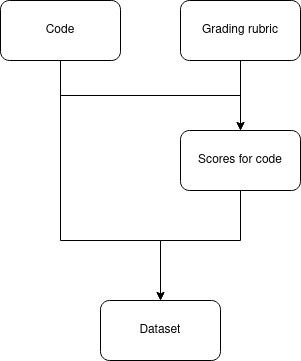
\includegraphics[scale=0.6]{data.png}
\caption{Data Annotation Flow}
\label{fig1}
\end{figure}

The score component for a value of 10 points was divided into two parts, \textbf{Design} (5 points) and \textbf{Functionality} (5 points). The subsequent pattern managed to cover the entirety of a code solution to provide a value balancing the code's design and functionality. 

For \textbf{Design}, considering each problem has its own set of parameters to satisfy, the grading rubric is adjusted based on this requirement. The parameters used for evaluating design is mentioned in Table II. Table III details the appropriate score to respective problems based on their necessary individual criteria for each different task.
        
        
\begin{table}[h!]
\centering
\renewcommand{\arraystretch}{1.3}
\begin{tabular}{|c|}
\hline
\textbf{Parameters} \\ \hline
Use of Variables \\ \hline
Modularity \\ \hline
Logic Application \\ \hline
Efficiency \\ \hline
\end{tabular}
\caption{Grading Parameters}
\label{tab:params}
\end{table}        
        
\begin{table*}[!ht]
\centering
\label{tab:my-table}
\begin{tabular}{l|cccc|}
\cline{2-5}
 & \multicolumn{4}{c|}{\textbf{Parameters}} \\ \hline
\multicolumn{1}{|c|}{\textbf{Program}} & \multicolumn{1}{l|}{\textit{\textbf{Use of Variables}}} & \multicolumn{1}{l|}{\textit{\textbf{Modularity}}} & \multicolumn{1}{l|}{\textit{\textbf{Logic application}}} & \multicolumn{1}{l|}{\textit{\textbf{Efficiency}}} \\ \hline
\multicolumn{1}{|l|}{First Negative Element in List} & \multicolumn{1}{c|}{1} & \multicolumn{1}{c|}{-} & \multicolumn{1}{c|}{2} & 2 \\ \hline
\multicolumn{1}{|l|}{Selection Sort} & \multicolumn{1}{c|}{1} & \multicolumn{1}{c|}{1} & \multicolumn{1}{c|}{1} & 2 \\ \hline
\multicolumn{1}{|l|}{Largest Element in List} & \multicolumn{1}{c|}{1} & \multicolumn{1}{c|}{-} & \multicolumn{1}{c|}{2} & 2 \\ \hline
\multicolumn{1}{|l|}{Unique Count of Characters} & \multicolumn{1}{c|}{1} & \multicolumn{1}{c|}{1} & \multicolumn{1}{c|}{1} & 2 \\ \hline
\end{tabular}
\caption{Grading Rubric}
\end{table*}
        
For \textbf{Functionality} the rubric mentioned in Table IV was followed to give a score out of 5. The correctness and completeness of the code was considered to grade the code submissions.

\begin{table}[h]
\centering
\begin{tabular}{|l|c|}
\hline
\textbf{\begin{tabular}[c]{@{}l@{}}Code's correctness\\ and \\ completeness\end{tabular}} & \multicolumn{1}{l|}{\textbf{Score}} \\ \hline
\begin{tabular}[c]{@{}l@{}}Perfectly correct\\ and complete\end{tabular}                     & 5                                   \\ \hline
\begin{tabular}[c]{@{}l@{}}Correct and complete\\ but can be improved\end{tabular}           & 4                                   \\ \hline
\begin{tabular}[c]{@{}l@{}}Complete but \\ partially incorrect\end{tabular}                  & 3                                   \\ \hline
\begin{tabular}[c]{@{}l@{}}Incomplete and\\ partially correct\end{tabular}                   & 2                                   \\ \hline
\begin{tabular}[c]{@{}l@{}}Incomplete and\\ totally incorrect\end{tabular}                   & 1                                   \\ \hline
\end{tabular}
\caption{Grading Rubric (Functionality)}
\label{grading_rub}
\end{table}

Ultimately a dataset compiled of code solutions and appropriate numeric score values (in a range of 0 to 10) was generated to be used for successive experimentation.

\subsection{Feature Extraction}

Following annotation of the dataset, feature extraction followed by feature selection is performed for optimal representation of code solutions as vectors for regression. The following series of steps were performed for extracting meaningful features from the dataset.

\begin{itemize}
        \item \textbf{Py2 to Py3 conversion}: The code solutions in the dataset are documented in python 2 version. To support extraction of features, python 2 to python 3 conversion was performed using the '2to3' module \cite{G}.
        \item \textbf{Abstract Syntax Tree (AST) representation}: After converting every program to python 3 format, the AST \cite{F} representation for each program was computed to derive appropriate features. The inbuilt python 'ast' module was used to get the ast representation of the student submissions. The ‘ast’ module provides a ‘parse()’ method which returns the AST representation of a code. A variety of features can be extracted from this ast representation with the help of ‘walk()’ function provided by the ‘ast’ module. The extracted features from the AST represenation are documented in Table VI. Other features derived from code are represented in Table V.
        
\end{itemize}

\begin{table}[h]
\centering
\begin{tabular}{|l|l|} 
\hline
return       & Count of 'return' statements in the code      \\ 
\hline
break        & Count of 'break' statements in the code       \\ 
\hline
continue     & Count of 'continue' statements in the code    \\ 
\hline
pass         & Count of 'pass' statements in the code        \\ 
\hline
assign       & Count of assignment operators in the code     \\ 
\hline
arith        & Count of arithmetic operators in the code     \\ 
\hline
comp         & Count of comparison operators in the code     \\ 
\hline
log          & Count of logical operators in the code        \\ 
\hline
cond         & Count of conditional operators in the code    \\ 
\hline
loop         & Count of 'for' and 'while' loops in the code  \\ 
\hline
\#lines      & Count of lines in the code                    \\ 
\hline
\end{tabular}

\caption{Features extracted from code}
\end{table}


\begin{table}[h]
\centering
\begin{tabular}{|l|l|} 
\hline 
\#fun                 & Count of function definitions in the code                                                                                      \\ 
\hline
\#fcall               & Count of function calls in the code                                                                                            \\ 
\hline
globals               & Count of globals variables in the code                                                                                         \\ 
\hline
\#lst                 & Count of lists and tuples in the code                                                                                          \\ 
\hline
\#var                 & \begin{tabular}[c]{@{}l@{}}Count of the variables in the code\\(Count of variables defined)\end{tabular}                       \\ 
\hline
\#var\_uses           & \begin{tabular}[c]{@{}l@{}}Count of variable uses in the code\\(Count of variables used in different statements)\end{tabular}  \\ 
\hline
\end{tabular}

\caption{Features extracted from AST} 
\end{table}


Ultimately a total of 17 features were extracted from the code and the AST representation of the code. 

\subsection{Feature Selection}

After extracting meaningful features from both code and AST representation (Table 5.8 \& Table 5.9), feature selection is performed for each problem considering feature sets for each problem are independent of each other and are problem dependent.

Firstly, the features that share the same value for all the code solutions are identified and removed to avoid redundancy. Once the redundant features are reduced, the number of features eventually reduces from 

\begin{itemize}
    \item 17 to 14 for 'Selection sort'
    \item 17 to 12 for 'The First negative element in the list'
    \item 17 to 12 for 'The Largest Element in List'
    \item 17 to 15 for 'The unique character count in a string task.'
\end{itemize}

Then, the best features are selected for each task according to how well they are correlated with the target variable. The \textbf{f\_regression} method \cite{H} returns the degree of correlation (F-statistic) between each feature and the target. 

The correlation F-statistic score of different features for the tasks are listed as tables below. After the F-statistic score is calculated, the features which have a appreciable influence on the target variable(score) are selected and the regressor model for each task is trained with the selected features.

\section{Design \& Architecture}

We propose a machine learning based student program evaluation system which represents student programs as a set of features extracted from the source programs and the AST representation of the source programs. Deep learning is purposely avoided since it would make the program's representation difficult to comprehend. The ML models are regression models which will output a score between 0 to 10 for each program submission. Feedback is provided to each program submission based on comparing the feature vector of the program with the average feature vector of 'good' programs.


\subsection{Training} 

\begin{figure}[h]
\centering
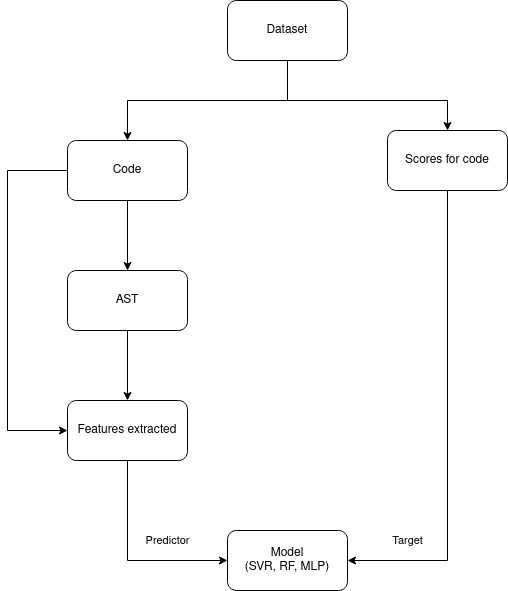
\includegraphics[width=0.48\textwidth]{./training.jpg}
\caption{Training}
\label{fig1}
\end{figure}

Dataset contains the code and corresponding scores for each of the student codes. Features from code were extracted by using two ways. Some features were extracted directly from the code. For the other features, the code was first transformed into an Abstract Syntax Tree(AST) then the features were extracted from the AST. The extracted features were used to train the model. Three models were trained separately: Support vector regressor, Random forest and Multi layer perceptron. The models trained were all regression models which were trained to predict the scores that should be given to the evaluated codes. 

\subsection{Deployment} 

\begin{figure}[h]
\centering
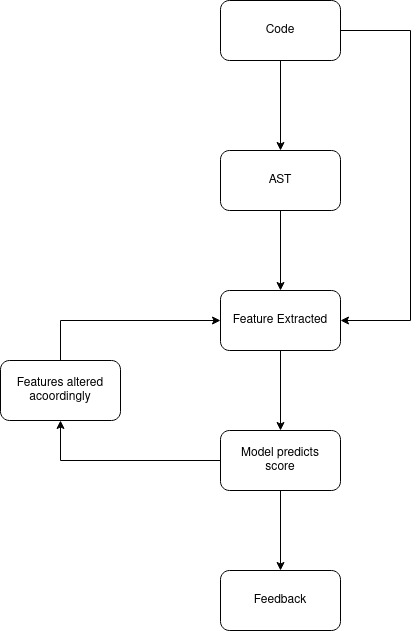
\includegraphics[width=0.48\textwidth]{./Deployment.jpg}
\caption{Deployment}
\label{fig1}
\end{figure}

The student code is input. Features are extracted from the code as explained in the section above. Some features are extracted from the code itself and the rest from an AST representation of the code. This feature set is input into the trained models from the previous section. The model predicts a score for the input code based on the feature set.

In order to avoid the need for a dataset with explicit feedback annotation, we use our model, trained on predicting design score, to evaluate how changes in program features would lead to a higher assessed score. Using the training data, we compute an average feature vector x of all the “good” programs. To generate feedback for a program, its feature vector is compared to the average.



\section{Algorithms}

After representing code solutions as feature vectors, the dataset was exported to perform training for machine learning models. The following models 

\begin{itemize}
    \item Support Vector Machine (SVM)
    \item Random Forest 
    \item Multi Layer Perceptron (MLP)
\end{itemize}

were employed for training. The detailed description of the mentioned algorithms are listed below. 

\subsection{Support Vector Machine}

Support Vector Machines (SVMs) are supervised learning models with associated learning algorithms that examine data for classification and regression in machine learning. Support Vector Regression \cite{D} is used to predict continuous values. The Support Vector Machine and Support Vector Regression are both based on the same premise (SVM). The goal of a support vector machine method is to find a hyperplane in an n-dimensional space that categorises data points clearly. Support Vectors are the data points on each side of the hyperplane that are closest to the hyperplane. These have an effect on the hyperplane's location and orientation, and so aid in the construction of the SVM. Following are the various key hyper parameters used in Support Vector Regression.


\begin{itemize}
    \item \textbf{Hyperplane}: A decision boundary that forecasts continuous output is known as a hyperplane. Support Vectors are the data points on each side of the hyperplane that are closest to the hyperplane. These are used to draw the essential line that depicts the algorithm's projected outcome.
    \item \textbf{Kernel}: A collection of mathematical functions that take input data and transform it into the required form. These are most commonly employed to locate a hyperplane in higher-dimensional space.
    \item \textbf{Boundary Lines}: These are the two lines that are drawn at an \textbf{$\epsilon$} (epsilon) distance around the hyperplane. It's used to separate the data points by a margin.
\end{itemize}

The best fit line or hyperplane with the most points is found using Support Vector Regression (SVR). The SVR, unlike other regression models, aims to fit the best line within a threshold value, rather than minimising the error between the real and projected value (the distance between the hyperplane and boundary line). As a result, we'll only consider points that fall inside the decision boundary and have the lowest error rate, or those that fall within the margin of tolerance. This results in a more accurate model.


\subsection{Random Forest}

Random forest is a Supervised Machine Learning Algorithm that is used widely in Classification and Regression problems. The functioning of Random Forest is contingent on three main factors, 

\begin{itemize}
\item \textbf{Ensemble Learning}: Ensemble learning is the process of using multiple models, trained over the same data, averaging the results of each model ultimately finding a more accurate predictive/classification result. The requirement for ensemble learning is that the errors of each model (in this case decision tree) are independent and different from tree to tree.

\item  \textbf{Decision Tree}: Decision Trees are used for both regression and classification problems. The goal is to create a model that predicts the value of a target variable by learning simple decision rules inferred from the data features. They start with the root of the tree and follow splits based on variable outcomes until a leaf node is reached and the result is given. 

\item \textbf{Bootstrapping}: Bootstrapping is the process of randomly sampling subsets of a dataset over a given number of iterations and a given number of variables. These results are then averaged together to obtain a more accurate result. 

The bootstrapping Random Forest algorithm \cite{B} combines ensemble learning methods with the decision tree framework to create multiple randomly drawn decision trees from the data, averaging the results to output a new result that often leads to strong predictions/classifications.

\end{itemize}

\subsection{Multi Layer Perceptron}

The Multi Layer Perceptron bases its fundamental design to the
interlinking of several neuron-like structures representing a Neural
Network (NN) architecture. Given $i = 0,1,\ldots,n$ where $n$ is the
number of inputs, the quantities $w_{i}$ are the weights of the
neuron. The inputs $x_{i}$ correspond to features or variables and the
output $y$ to their prediction/estimation.

The weighting step involves the multiplication of each input feature value by its weight ${w_ix_i}$ and then they are summed together $(x_{0}w_{0} + x_{1}w_{1} + ... + x_{n}w_{n})$. In the transfer step, an activation function f (also called a transfer function) is applied to the sum producing an output $y$
presented as: 

\begin{equation}
    y = f(z)\;and\;z = \sum_{i=0}^{n} w_{i}x_{i}
\end{equation}

wherein $x_{0} = 0$, $w_{0}$ is the bias and $y$ is the output. The
activation function can be of the form of Unit step, Linear or
Logistic operation.

For $n$
dimensions, the function is a hyperplane with equation:

\begin{equation}
    \sum_{i=0}^{n} w_{i}x_{i} = 0
\end{equation}

The goal of learning is to minimise a cost function, which is commonly a square error between the known and estimated vectors, in order to optimise the weights. The best weight vector can be determined using optimization techniques such as the gradient descent algorithm. The algorithm eventually converges on a solution that reaches an operational configuration network. The perceptron and single layer perceptron, on the other hand, do not address the nonlinearly separable problem.

To solve this problem, Multi Layer Perceptron (MLP) architecture is
created by aggregating layers of perceptrons wherein the output of one
layer acts as the input of another layer. Multi Layer Perceptron
\cite{C} is a feedforward neural network that consists of three
layers, the input layer, the hidden layer and the output
layer. Figure~4.7 presents an MLP with two inputs (blue), two hidden
layers (grey) and one output (red).

The input signal to be processed is received by the input layer. The output layer is responsible for tasks such as prediction and categorization. The true computational engine of the MLP is an arbitrary number of hidden layers inserted between the input and output layers. In an MLP, data flows from input to output layer in the forward direction, similar to a feed forward network. The weights of the neurons in the MLP can be adjusted by propagating errors from layer to layer, starting with the output layer and going backwards, using the back propagation learning process. MLPs can tackle issues that aren't linearly separable and are designed to approximate any continuous function.

\section{Implementation}

The implementation of models was performed using the Scikit-Learn library \cite{E}. For each code submission task, the dataset was split in the ratio 70:30 for training and testing. With respective to the hyper-parameters initialized for the individual models, 

\begin{itemize}
    \item The MLP regressor model was initialised with a single hidden layer with 100 neurons. The maximum iterations parameter was set to 5000. 
    \item The Random Forest Regressor was initialised with 100 estimators(decision trees).
    \item The Support Vector Regressor was initialised with radial basis function kernel.
\end{itemize} 

% Talk about train test split

\subsection{Metrics}
 

\subsubsection{\textbf{Mean Absolute Error (MAE)}}

\[ MAE = \frac{\sum_{i=1}^{n}|t_i-y_i|}{n} \]

MAE is the mean of magnitude of difference between true value '$t_{i}$' and prediction '$y_{i}$' of 'n' observations.

\subsubsection{\textbf{Root Mean Absolute Error (RMSE)}}

\[ RMSE = \sqrt{\frac{\Sigma_{i=1}^{n}{|t_i-y_i|}^2}{n}} \]

RMSE is the square root of the mean of residuals (difference between between true value '$t_{i}$' and prediction '$y_{i}$') of 'n' observations 

\subsection{Results}

The observed values of MAE and RMSE obtained for the different set of tasks are reported in Tables VII - X. The values enclosed in brackets report scores observed with feature selection and the values not enclosed in brackets report scores observed without feature selection. 


\begin{table}[h]
\centering
\begin{tabular}{|c|c|c|}
\hline
\textbf{Model} & \textit{\textbf{MAE}} & \textit{\textbf{RMSE}} \\ \hline
\textbf{SVM}   & 1.35 \textbf{(1.27)}           & 1.94 \textbf{(1.84)}            \\ \hline
\textbf{MLP}   & 2.18 \textbf{(3.29)}           & 2.60 \textbf{(3.61)}             \\ \hline
\textbf{RF}    & 1.18 \textbf{(1.17)}           & 1.87 \textbf{(1.83)}            \\ \hline
\end{tabular}
\caption{Results - Selection Sort}
\label{tab:selsort}
\end{table}


\begin{table}[h]
\centering
\begin{tabular}{|c|c|c|}
\hline
\textbf{Model} & \textit{\textbf{MAE}} & \textit{\textbf{RMSE}} \\ \hline
\textbf{SVM}   & 2.13 \textbf{(2.11)}           & 2.97 \textbf{(2.99)}            \\ \hline
\textbf{MLP}   & 3.02 \textbf{(3.13)}           & 3.80 \textbf{(3.90)}            \\ \hline
\textbf{RF}    & 1.60 \textbf{(1.64)}           & 2.15 \textbf{(2.20)}            \\ \hline
\end{tabular}
\caption{Results - First Negative Item in List}
\label{tab:first-neg}
\end{table}

\begin{table}[h]
\centering
\begin{tabular}{|c|c|c|}
\hline
\textbf{Model} & \textit{\textbf{MAE}} & \textit{\textbf{RMSE}} \\ \hline
\textbf{SVM}   & 2.19 \textbf{(1.89)}           & 2.85 \textbf{(2.35)}            \\ \hline
\textbf{MLP}   & 2.73 \textbf{(3.28)}           & 3.61 \textbf{(4.23) }           \\ \hline
\textbf{RF}    & 1.51 \textbf{(1.47)}           & 2.10 \textbf{(2.07)}            \\ \hline
\end{tabular}
\caption{Results - Largest Item in List}
\label{tab:larg-list}
\end{table} 

\begin{table}[h]
\centering
\begin{tabular}{|c|c|c|}
\hline
\textbf{Model} & \textit{\textbf{MAE}} & \textit{\textbf{RMSE}} \\ \hline
\textit{SVM} & 2.63 \textbf{(2.68)} & 3.19 \textbf{(3.23)} \\ \hline
\textit{MLP} & 3.11 \textbf{(2.71)} & 3.93 \textbf{(2.86)} \\ \hline
\textit{RF} & 2.16 \textbf{(2.19)} & 2.62 \textbf{(2.64)} \\ \hline
\end{tabular}
\caption{Unique Characters count in a string}
\label{tab:my-table}
\end{table}

\subsection{Inference}

The number of features in the dataset is a relatively small (only 17
features). And with feature selection, the number reduces even
further.  As mentioned earlier, various decision tree together comprise a random forest regression model. Since decision trees output a score based on feature value conditions(for instance, when functions = 3 for selection sort task, the decision tree will output a better score) and the outputs of the decision trees are ensembled, the random forest regression algorithm fits well with this data and outperforms the other two models in this case.

Also, while multi layer perceptron regressor and linear support vector regressor can output a score greater than 10 or lesser than 0, random forest regressor always outputs a score in the range of 0 to 10. This characteristic of random forest regressor is accounted by the decision trees which form the regressor. Since MLP regressor trains through backpropagation and support vector regressor tries to find the best hyperplane which contains maximum number of points, these models may output a score greater than 10 as far as the conditions are satisfied. But in the case of random forest regressor, the model outputs a score based on the ensembling of various decision trees. The maximum score that can be awarded will be set as 10 and when a particular code submission passes all conditions(conditions are based on different feature values), that program will be graded with a score of 10. 

\section{Feedback Generation}

After prioritizing the best regression models for each problem, we move on to using the selected model for generating feedback. The feedback generation process follows a cyclic information flow where the model is verified each time for a change depending on the input change and the corresponding change is reflected as feedback. The following subsections detail on the process of how constructive feedback is generated. 

\subsection{Golden Feature Vector}

    The Golden feature vector $F$ is the best feature vector that is calculated for each problem. In retrospect, the golden feature vector is the average of feature vectors of all code solutions submitted for the program that have score greater than or equal to an empirically decided threshold. 

At any instance, the Golden feature vector represents the correct and accurate code solutions for a particular problem. The goal of this vector is to act as a comparison tool for feature vectors that require feedback/optimization. 

\subsection{Algorithm}

Now, to generate feedback for a particular target program $x$ with $x_{i}$ features where i = 0,1,2...n (n - number of features) - we perform an iterative process of replacing one of the features $x_{i}$ with the corresponding feature value $X_{i}$ from the program's Golden Feature vector $F$. Now, the new modified feature vector is passed as input into the regression model. 

\begin{itemize}

    \item If the output score improves after replacement, now we compare $x_{i}$ and $X_{i}$.

        \begin{itemize}
                \item If $x_{i}$ $>$ $X_{i}$ - Feedback to decrease that particular feature in the program is advised. 
                \item If $x_{i}$ $<$ $X_{i}$ - Feedback to increase the particular feature in the program is advised.
        \end{itemize}
        
    \item If the output score decreases after replacement, we consider the next feature in $x_{i}$
    
    \item The above process is iterated until all the n features have been considered. 

\end{itemize}

In each iteration the goal of the algorithm is to make the target feature vector closer to the golden feature vector. Thereby the changes that are suggested as feedback are inferred to be optimization changes for the target vector and constructive feedback is provided. 

\section{Conclusion }

We proposed a pipeline for grading a student code submission out of 10
which will also provide appropriate feedback to improve the code. The student programs were represented using 17 features which were retrieved from the submitted codes and from the AST representation of the codes. Feature set for each coding
assignment was optimised via feature selection. The initial dataset
created by us was used to train three regressor models such as Linear SVR, MLP regressor and Random Forest
Regressor. The Random Forest regressor was shown to be the most
effective for this problem statement. The Random Forest Regressor model
has a MAE of 1.7 and RMSE of 2.3.

Furthermore, our technique delivers personalised feedback for a program by comparing its feature vector with the average feature vector of the "excellent" programs submitted by students.Whenever a student submits a
code, he will be given feedback instantly to help him improve his
code.  Students can also view the best code submission after the
assignment deadline. The Streamlit framework was used to deploy this
pipeline as a web app.


\begin{thebibliography}{99}
  \bibliographystyle{plain}
  
\bibitem[1]{A} Azcona, D., Arora, P., Hsiao, I. H., \& Smeaton, A. (2019, March). user2code2vec: Embeddings for profiling students based on distributional representations of source code. In Proceedings of the 9th International Conference on Learning Analytics \& Knowledge (pp. 86-95).


\bibitem[2]{T}Orr, J. Walker, and Nathaniel Russell. "Automatic Assessment of the Design Quality of Python Programs with Personalized Feedback." arXiv preprint arXiv:2106.01399 (2021).

\bibitem[3]{G} 2to3 - Automated Python 2to3 code translation -https://docs.python.org/3/library/2to3.html


\bibitem[4]{F} AST module Python 3.10.4- https://docs.python.org/3/library/ast.html


\bibitem[5]{H} Jović, Alan, Karla Brkić, and Nikola Bogunović. "A review of feature selection methods with applications." 2015 38th international convention on information and communication technology, electronics and microelectronics (MIPRO). Ieee, 2015.

\bibitem[6]{E} Scikit-learn: Machine Learning in Python, Pedregosa et al., JMLR 12, pp. 2825-2830, 2011.


\bibitem[7]{D} Drucker, Harris, et al. "Support vector regression machines." Advances in neural information processing systems 9 (1996).

\bibitem[8]{B} Breiman, L. (2001). “Random forests - Machine Learning” 45, 5-32.

\bibitem[9]{C} Murtagh, Fionn. "Multilayer perceptrons for classification and regression." Neurocomputing 2.5-6 (1991): 183-197.


\bibitem[10]{I} Uri Alon, Meital Zilberstein, Omer Levy, and Eran Yahav. 2018. A general path-based representation for predicting program properties. arXiv preprint arXiv:1803.09544 (2018).

\bibitem[11]{J} Maxim Rabinovich, Mitchell Stern, and Dan Klein. 2017. Abstract syntax networks for code generation and semantic parsing. arXiv preprint arXiv:1704.07535 (2017).

\bibitem[12]{K} Veselin Raychev, Martin Vechev, and Eran Yahav. 2014. Code completion with statistical language models. In Acm Sigplan Notices, Vol. 49. ACM, 419–428.

\bibitem[13]{L} Miltiadis Allamanis, Hao Peng, and Charles Sutton. 2016. A convolutional attention network for extreme summarization of source code. In International Conference on Machine Learning. 2091–2100.


\bibitem[14]{M} Lili Mou, Ge Li, Yuxuan Liu, Hao Peng, Zhi Jin, Yan Xu, and Lu Zhang. 2014. Building program vector representations for deep learning. arXiv preprint arXiv:1409.3358 (2014).

\bibitem[15]{N} Chris Piech, Jonathan Huang, Andy Nguyen, Mike Phulsuksombati, Mehran Sahami, and Leonidas Guibas. 2015. Learning program embeddings to propagate feedback on student code. In Proceedings of the 32nd International Conference on International Conference on Machine Learning-Volume 37. JMLR. org, 1093–1102.

\bibitem[16]{O} Benjamin Paaßen, Barbara Hammer, Thomas William Price, Tiffany Barnes, Sebastian Gross, and Niels Pinkwart. 2017. The Continuous Hint Factory-Providing Hints in Vast and Sparsely Populated Edit Distance Spaces. arXiv preprint arXiv:1708.06564 (2017).


\bibitem[17]{P} Sebastian Gross, Bassam Mokbel, Benjamin Paaßen, Barbara Hammer, and Niels Pinkwart. 2014. Example-based feedback provision using structured solution spaces. International Journal of Learning Technology 10 9, 3 (2014), 248–280.

\bibitem[18]{Q} Lili Mou, Ge Li, Lu Zhang, Tao Wang, and Zhi Jin. 2016. Convolutional Neural Networks over Tree Structures for Programming Language Processing.. In AAAI, Vol. 2. 4.

\bibitem[19]{R} Sebastian Proksch, Sven Amann, Sarah Nadi, and Mira Mezini. 2016. A dataset of simplified syntax trees for C. In Proceedings of the 13th International Conference on Mining Software Repositories. ACM, 476–479.

\bibitem[20]{S} Pylint.org. Pylint - code analysis for python. https://pylint.org.

\end{thebibliography}



\end{document}
